\chapter{Introduzione e Contesto}
L'attuale generazione della tecnologia World Wide Web, denominata \textit{"Web2"}, è caratterizzata da una maggiore interattività e partecipazione degli utenti rispetto alla precedente generazione, detta \textit{"Web1"}. In genere, con il termine Web2, si denota la transizione dalla semplice navigazione di siti web all'utilizzo, da parte degli utenti della rete, di servizi e applicazioni interattive, come ad esempio: i social network, le piattaforme di streaming e gli e-commerce.

Questa seconda generazione è anche caratterizzata da un \textit{problema di centralizzazione}, il quale consiste nel fatto che molte delle informazioni e dei dati che circolano in rete sono gestiti da un numero ristretto di grandi aziende. Ciò può portare a problemi di privacy, sicurezza e libertà d'espressione, in quanto queste aziende possono utilizzare i dati degli utenti per fini commerciali o per influenzare l'accesso a determinate informazioni. Inoltre, la centralizzazione introduce problemi di dipendenza e vulnerabilità, in quanto un'unica entità ha il controllo sui dati e sui servizi forniti, la quale, se attaccata attraverso vulnerabilità, può essere soggetta al furto di una grande mole di dati sensibili.

La prossima generazione, denominata \textit{"Web3"}, punta a risolvere questo problema attraverso la decentralizzazione e la creazione di applicazioni e servizi che non dipendono da un'unica entità o autorità centrale, ma che sono gestiti da una rete di nodi distribuiti. In questo modo, si mira a creare una rete più equa, sicura e resiliente, dove gli utenti hanno il controllo dei propri dati e delle proprie informazioni.\\
\\
Di seguito in questo capitolo vengono presentati i concetti fondamentali del Web3, il tema d'interesse e il lavoro svolto per la tesi e la struttura generale della tesi.

\section{Le blockchain}
Le blockchain sono una tecnologia di registro digitale distribuito che consente la creazione di una \textit{rete peer-to-peer} senza la necessità di intermediari. Ciò significa che le informazioni possono essere scambiate direttamente tra gli utenti senza la necessità di un'autorità centrale.
Una blockchain è formata da una serie di blocchi, ognuno dei quali contiene delle transazioni. Tali blocchi vengono inseriti cronologicamente in catena attraverso il consenso degli altri peer, creando di fatto un registro:

\begin{itemize}
	\item \textit{condiviso}: poiché viene replicato in ogni nodo della rete;
	\item \textit{immutabile}: in quanto una volta inserito un blocco, quest'ultimo non potrà essere eliminato o modificato;
\end{itemize}
Queste caratteristiche rendono le blockchain adatte per la creazione di un Internet decentralizzato in cui gli utenti hanno maggiore sicurezza, trasparenza e autonomia.

\subsection{La blockchain Ethereum}

\begin{wrapfigure}{r}{0.20\textwidth}
	\centering
	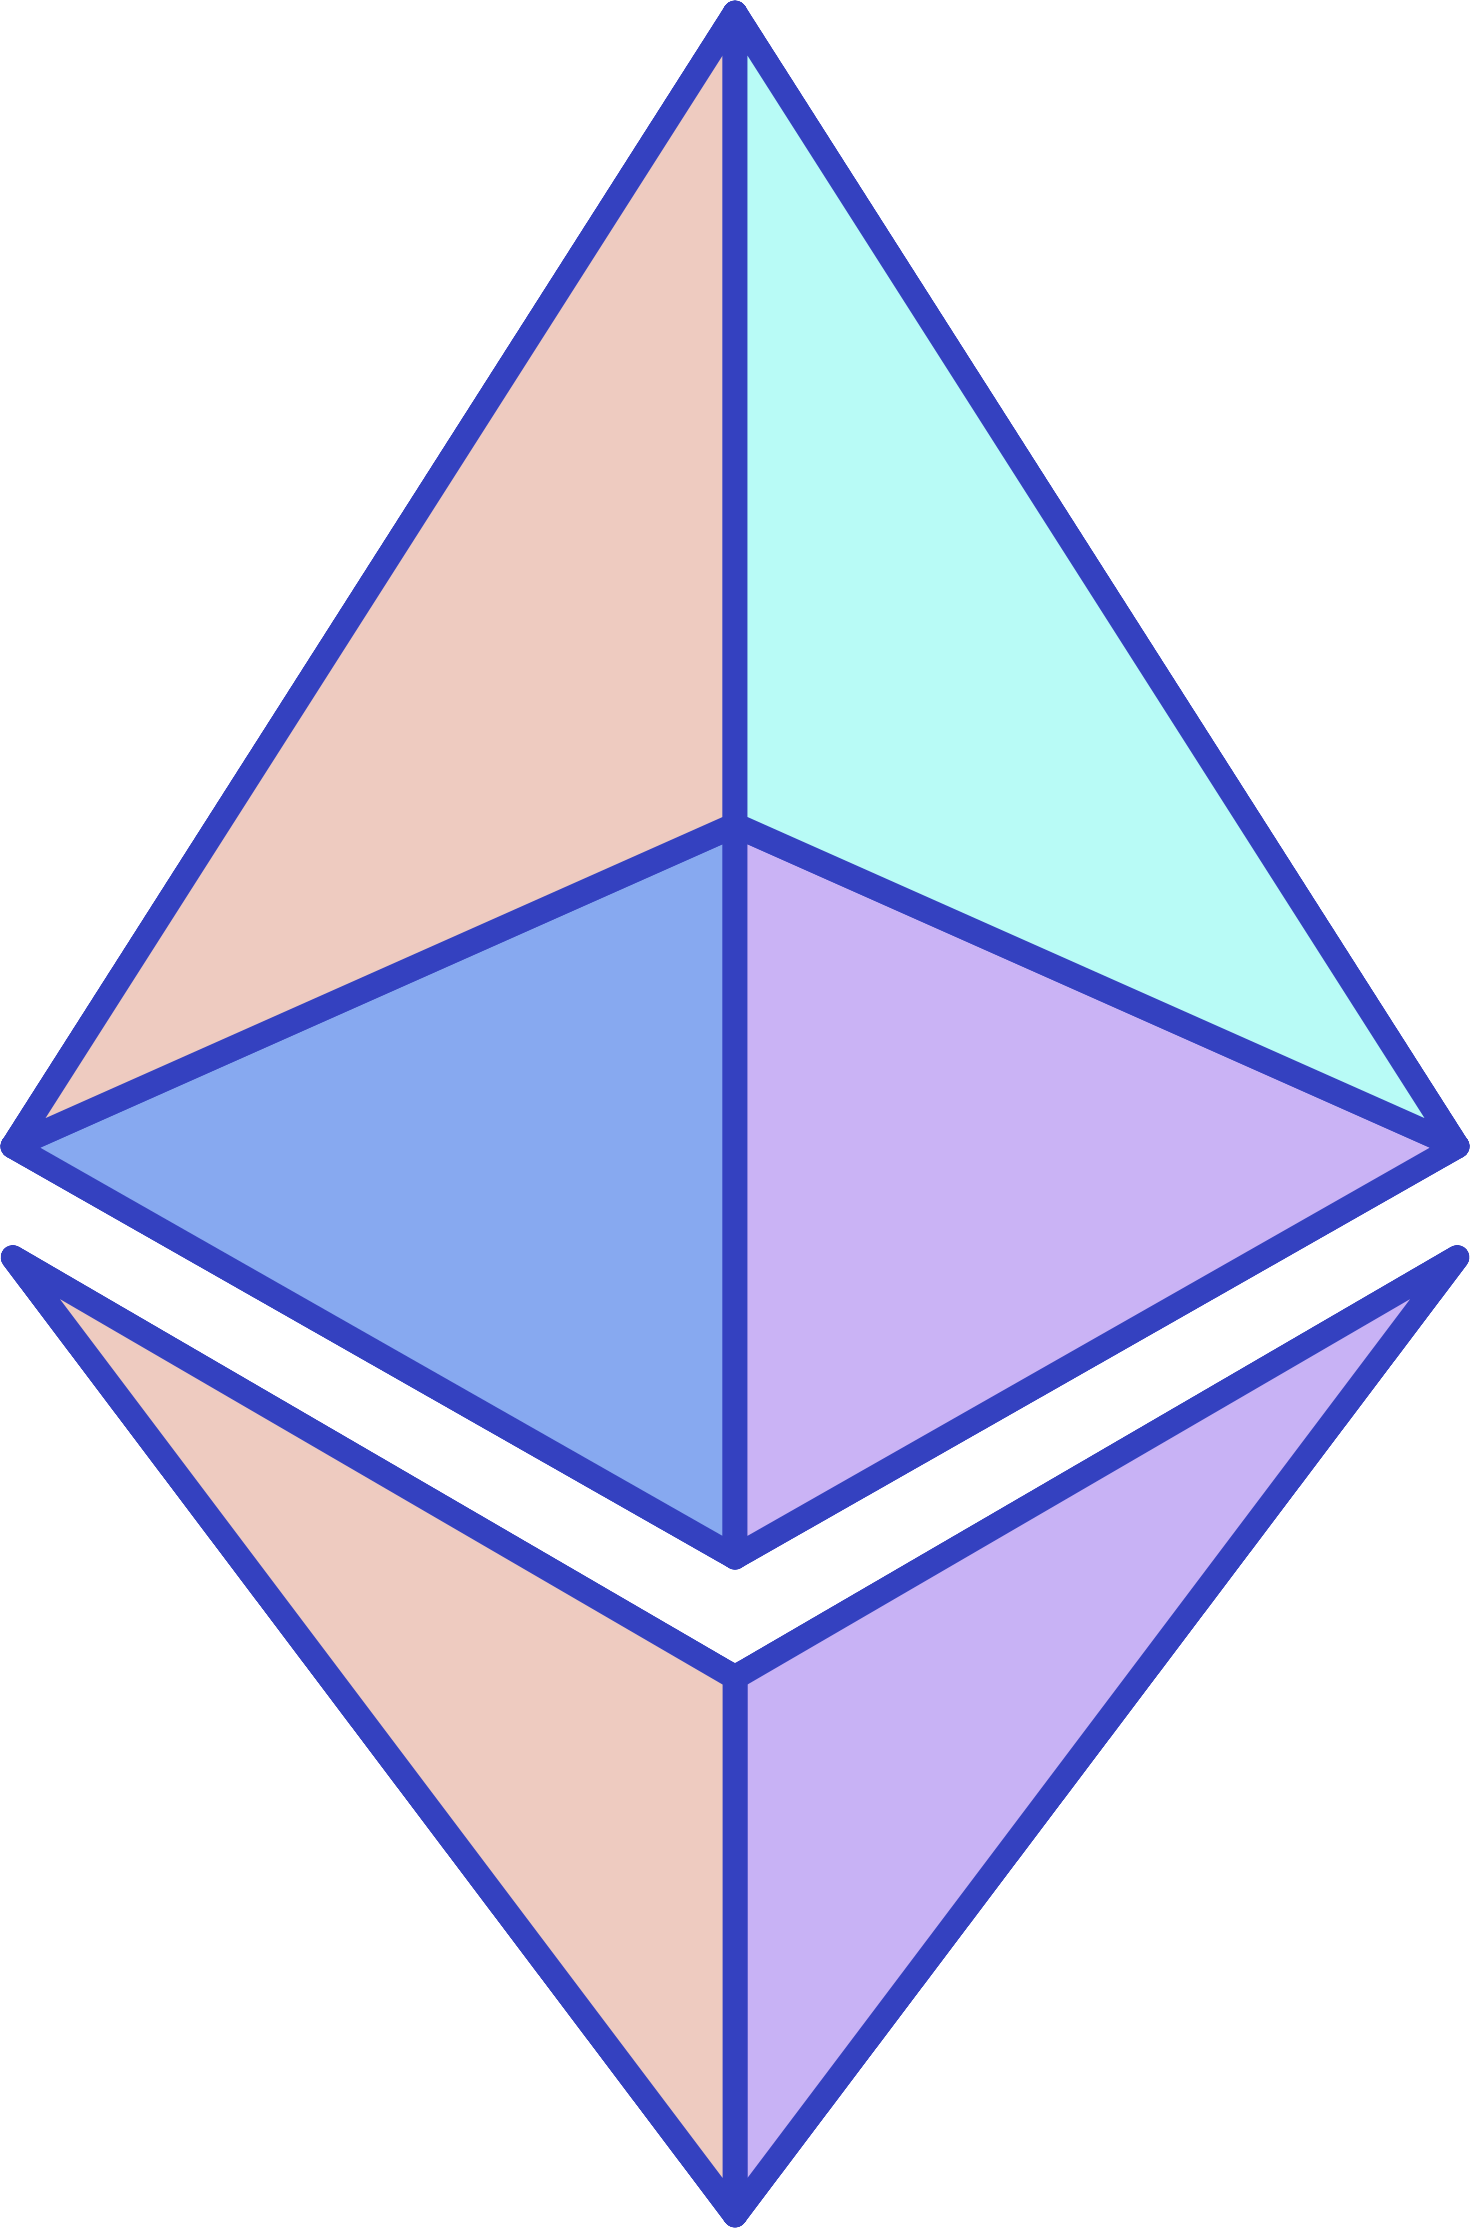
\includegraphics[scale=0.03]{ethereum-logo}
\end{wrapfigure}

Ethereum\cite{ethereum} è una blockchain open-source, lanciata nel 2015 da Vitalik Buterin e altri sviluppatori, velocemente diventata una delle più grandi e utilizzate blockchain al mondo. Rispetto alla blockchain Bitcoin, una delle differenze chiave consiste nel fatto che Ethereum è programmabile, ovvero offre agli sviluppatori una piattaforma per la creazione e l'esecuzione di smart-contract, con i quali è possibile creare applicazioni decentralizzate, denominate \textit{dApp}, utilizzabili per diversi scopi, come la gestione di beni digitali e la creazione di mercati decentralizzati. Ethereum ha una propria criptovaluta, denominata \textit{"Ether"}, usata per pagare per certe attività sulla rete di Ethereum.

\section{Gli Smart-Contract}

\begin{wrapfigure}{l}{0.20\textwidth}
	\centering
	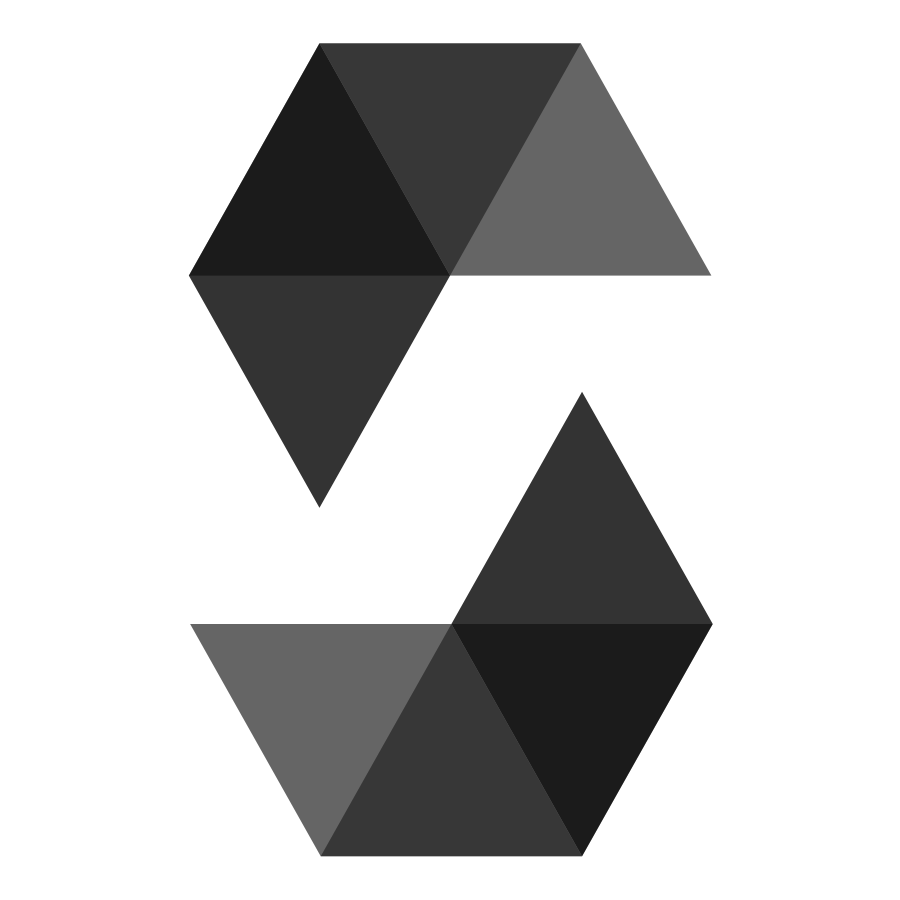
\includegraphics[scale=0.1]{solidity-logo}
\end{wrapfigure}

Ethereum permette la creazione e la gestione di smart-contract, una forma di contratto digitale automatizzato che si esegue automaticamente, all'interno della rete, quando determinate condizioni sono soddisfatte. Gli smart-contract consentono la creazione di accordi automatici tra le parti in modo da ridurre i tempi di elaborazione e i costi associati alle transazioni tradizionali. Questi contratti intelligenti sono scritti da un programmatore in un linguaggio di programmazione denominato \textit{"Solidity"}\cite{solidity} che consente la definizione di regole e logiche specifiche che vengono eseguite in una blockchain. Come in ogni sviluppo software, durante lo sviluppo di uno smart-contract si può incorrere in vulnerabilità e problemi di sicurezza, che permetterebbero a un attaccante di compromettere il contratto e causare danni ingenti e irreparabili. Per tale motivo, con il passare del tempo, i programmatori hanno ideato delle soluzioni ai problemi noti, definendo di fatto dei design pattern specifici per smart-contract.

\section{Il tema e lo sviluppo della Tesi}
Usando come riferimento la relativa pubblicazione scientifica e i consigli della comunità di programmatori Solidity, disponibili al momento della stesura di questa tesi, si prefigge l'obiettivo di studiare, analizzare e documentare quali \textit{design pattern} siano attualmente utilizzati nello sviluppo degli smart-contract della blockchain Ethereum.

L'obiettivo fissato si fonda sulla tecnica di \textit{analisi statica} (nota anche come \textit{"static analysis"} o \textit{"code analysis"}), una tecnica che si occupa di esaminare il codice sorgente di un software senza eseguirlo effettivamente, con lo scopo di identificare eventuali vulnerabilità, bug, inefficienze o altri problemi di qualità del codice. 

Al fine di conseguire l'obiettivo, si propone lo sviluppo di un applicativo software capace di eseguire automaticamente l'analisi statica sul codice sorgente di uno smart-contract, scritto in Solidity, fornito in input, rilevare quali design pattern siano utilizzati e restituire in output tali informazioni all'utente finale. 


\section{Struttura della Tesi}
Di seguito vengono illustrati gli argomenti trattati in ogni capitolo presente:
\begin{itemize}
	\item Nel \textit{capitolo 2} vengono introdotti gli strumenti utilizzati per lo svolgimento del tema della tesi;
	\item Nel \textit{capitolo 3} vengono descritti i design pattern individuati nello studio dell'attuale divulgazione scientifica;
	\item Nel \textit{capitolo 4} viene presentato il software di analisi statica automatica sviluppato;
	\item Nel \textit{capitolo 5} vengono riportati i risultati;
	\item Nell'\textit{appendice} vengono riportati i codici di riferimento dei design pattern usati per lo sviluppo del software;
\end{itemize}